\documentclass[xcolor={usenames,dvipsnames},handout]{beamer}
%\documentclass[draft]{beamer}


\usepackage[dvipsnames]{xcolor}



\usepackage[utf8]{inputenc}
\usepackage[T1]{fontenc}
\usetheme{MOKAbeamer}

%\usepackage[french]{babel}



\usepackage{tikz}

%\usepackage[draft]{animate}
\usepackage{animate}
\usepackage{ifthen}
\usepackage{filecontents}
\usepackage{stmaryrd}
\usepackage{listliketab}

\usepackage{multirow}

\usetikzlibrary{calc}
\usepackage{pifont}
\usepackage{mystyle}

\usepackage{tabularx}

\usepackage{algorithm,algorithmic}

\usepackage{standalone} % pour compiler les tikz -> input
\definecolor{vertsombre}{rgb}{0.0,0.5,0.0}
\usepackage{array}
\newcolumntype{M}{>{\centering\arraybackslash} m{0.5cm} }

\newcommand{\cyte}[1]{{\scriptsize\color{domcolor}#1}}
\newcommand{\cyteb}[1]{{\footnotesize\color{white}#1}}

%Pour ne pas compter les derniers slides
\newcommand{\backupbegin}{
   \newcounter{finalframe}
   \setcounter{finalframe}{\value{framenumber}}
}
\newcommand{\backupend}{
   \setcounter{framenumber}{\value{finalframe}}
}



%\newtheorem{theorem}{Theorem}[chapter]
%\newtheorem{lemma}[theorem]{Lemma}
\newtheorem{prop}[theorem]{Proposition}
%\newtheorem{corollary}[theorem]{Corollary}
%\newtheorem{definition}[theorem]{Definition \rm}
%\newtheorem{definition}[theorem]{Definition}
\newtheorem{remark}[theorem]{Remark}

%Debug boxes
\showboxdepth=5
\showboxbreadth=5


\newcommand{\nfb}[1]{\begin{frame}[allowframebreaks]#1\end{frame}}


\begin{document}
\title[]{Introduction to Machine learning}
\author[]{Sylvain Le Corff}
\date{}

\begin{frame}[plain]
\titlepage
\end{frame}


%%%%%%%%%%%%%%%%%%%%%%%%%%%%%%%%%%%%%%
%%%%%%%%%% PRELIMINARY %%%%%%%%%%%%%%%%%
%%%%%%%%%%%%%%%%%%%%%%%%%%%%%%%%%%%%%%


\begin{frame}
\structure{Prerequisites}: basics of probability and statistics.

\vspace{.5cm}

\structure{Objectives}:  

\vspace{.2cm}

$\rightharpoondown$ Learn and apply the \alert{fundamental concepts} of statistical learning; 

\vspace{.3cm}

$\rightharpoondown$ Understand the \alert{basic theory} underlying data science;

\vspace{.3cm}


$\rightharpoondown$ Implement (\alert{Python}) the most classical \alert{learning} algorithms;

\vspace{.3cm}

$\rightharpoondown$ Be able to read current research books and papers.

\vspace{.5cm}

\structure{This course}: 

\vspace{.2cm}

$\rightharpoondown$ \alert{4h of lecture/TD/TP per week}; 

\vspace{.3cm}

$\rightharpoondown$ \alert{Evaluation}: 1/4 QCM en cours + 3/4 exam.

\end{frame}


%%%%%%%%%%%%%%%%%%%%%%%%%%%%%%%%%%%%%%
%%%%%%%%%  INTRO %%%%%%%%%%%%%%%%%%%%%%%
%%%%%%%%%%%%%%%%%%%%%%%%%%%%%%%%%%%%%%

\begin{frame}{Introduction to machine learning}
\tableofcontents
\end{frame}



\section{Some applications}







\begin{frame}{Computer vision}
\begin{figure}
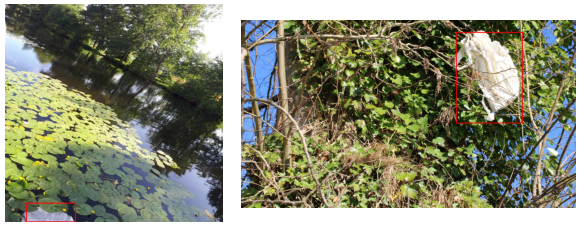
\includegraphics[width=0.7\linewidth]{plastic}
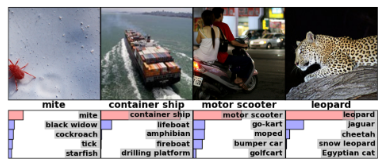
\includegraphics[width=0.7\linewidth]{image_classif}
\caption{Detection of plastic trash in videos, image classification.  {\tiny \href{https://proceedings.neurips.cc/paper/2012/file/c399862d3b9d6b76c8436e924a68c45b-Paper.pdf}{\structure{(ImageNet, Krizhevsky et al., 2012)}}},   {\tiny \href{PlasticTrash}{\structure{(Chagneux et al. 2022)}}}.}
\end{figure}
\end{frame}

\begin{frame}{Computer vision}
\begin{figure}
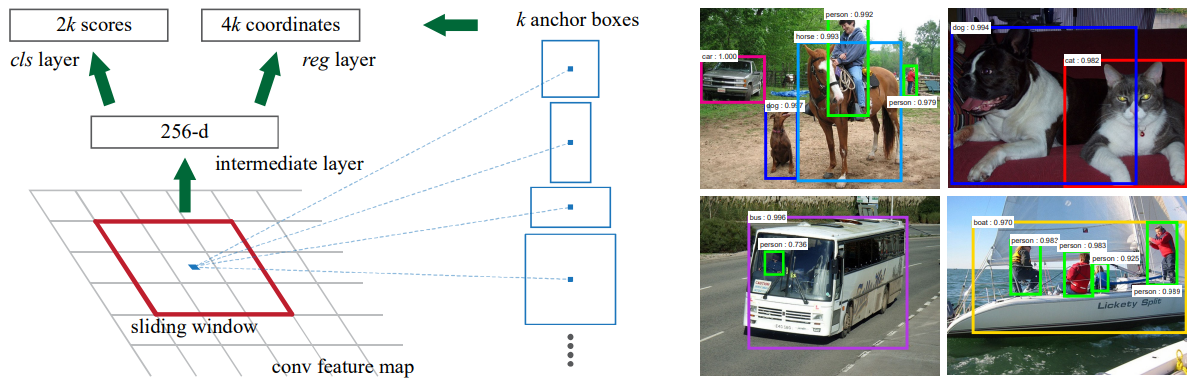
\includegraphics[width=0.9\linewidth]{image_bbox}
\caption{Automatic detections using Region Proposal Network (bounding box design). {\tiny \href{https://papers.nips.cc/paper/2015/hash/14bfa6bb14875e45bba028a21ed38046-Abstract.html}{\structure{(Faster-RCNN, Ren et al. 2015)}}}. Code is available at \url{https://github.com/ShaoqingRen/faster_rcnn}.}
\end{figure}
\end{frame}

\begin{frame}{Vision + Natural Language Processing}
\begin{figure}
\includegraphics[width=0.7\linewidth]{Mutan}
\caption{Visual Question Answering (VQA) tasks. {\tiny \href{https://arxiv.org/pdf/1705.06676.pdf}{\structure{(Mutan, Ben-Younes et al. 2017)}}}.}
\end{figure}
\end{frame}

\begin{frame}{Medical applications}
\begin{figure}
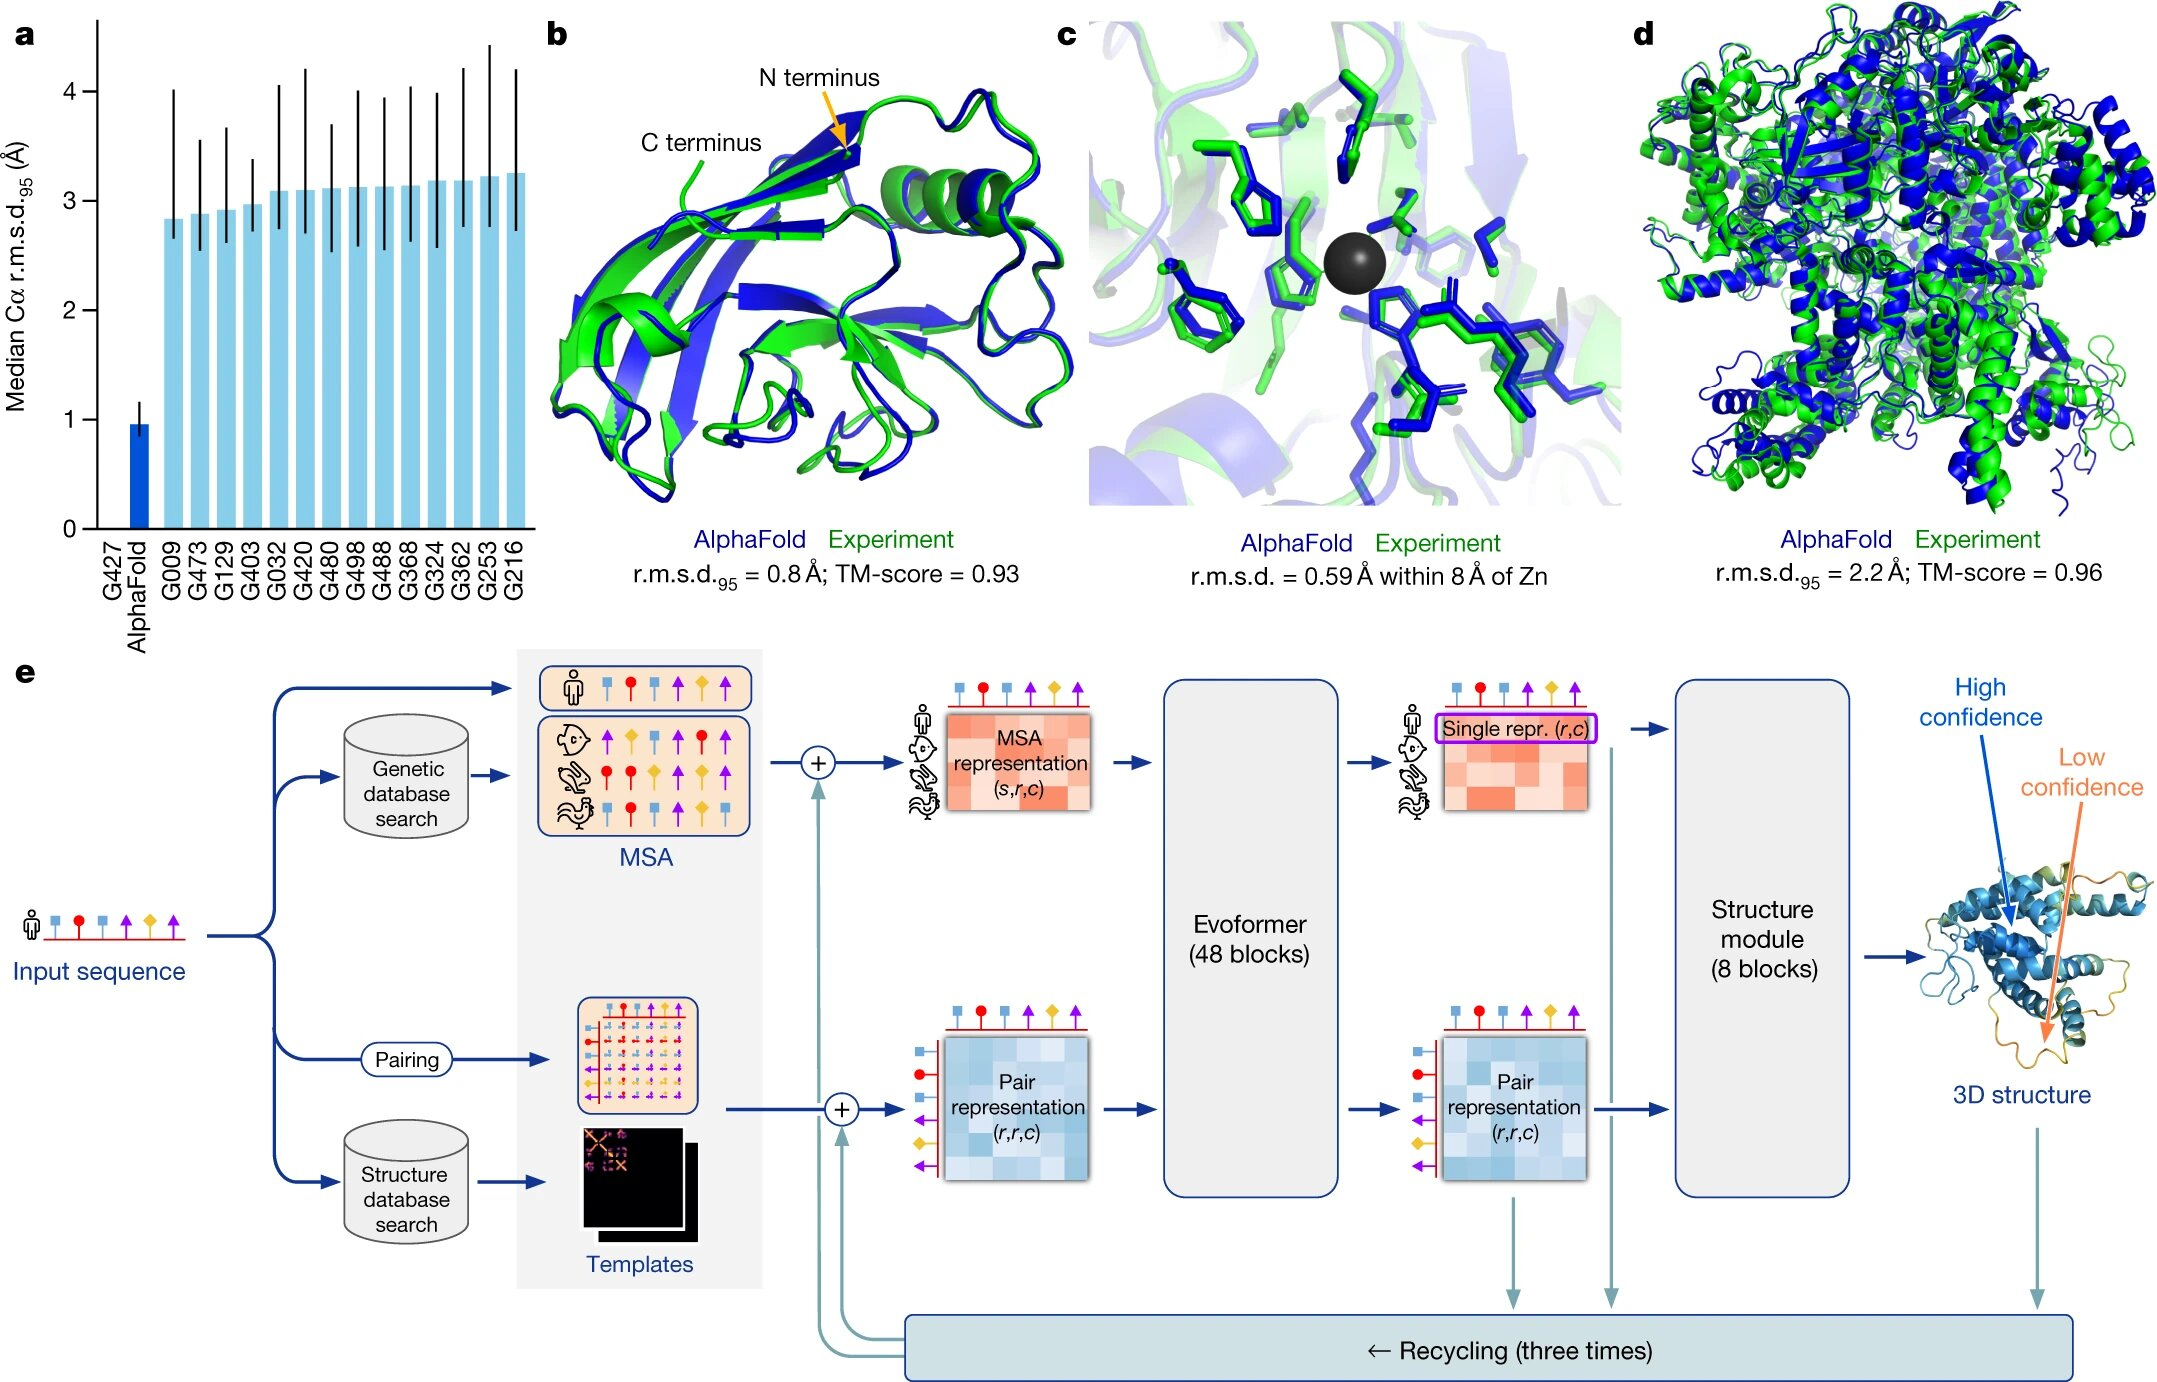
\includegraphics[width=0.9\linewidth]{alphafold}
\caption{Predicting the three-dimensional structure that a protein will adopt based solely on its amino acid sequence—the structure prediction component of the "protein folding problem". Performance of AlphaFold on the CASP14 dataset. {\tiny \href{https://www.nature.com/articles/s41586-021-03819-2}{\structure{(AlphaFold, Jumper et al. 2022)}}}.}
\end{figure}
\end{frame}

\begin{frame}{Challenges - reduce GHG emissions from cities}
\begin{figure}
\centering
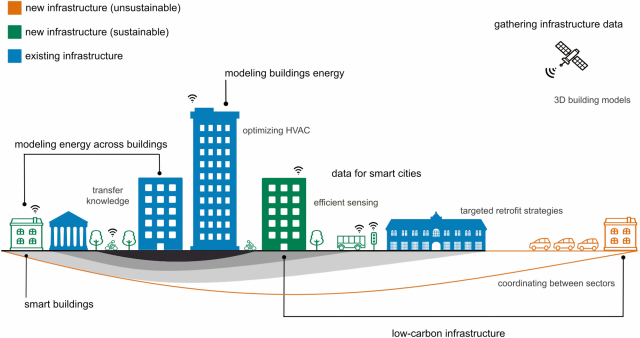
\includegraphics[width=0.8\linewidth]{smart_city}
\caption{Selected opportunities to reduce GHG emissions from buildings and cities using ML.   {\tiny\href{https://dl.acm.org/doi/full/10.1145/3485128}{\structure{(Tackling Climate Change with Machine Learning, Rolnick et al. 2022)}}}.}
\end{figure}
\end{frame}

\begin{frame}{Challenges - reduce GHG emissions from land use}
\begin{figure}
\centering
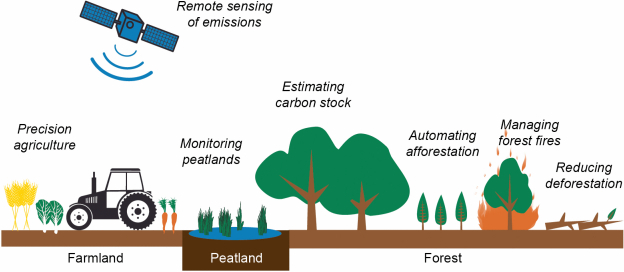
\includegraphics[width=0.8\linewidth]{smart_agr}
\caption{Selected opportunities to reduce GHG emissions from land use using ML.  {\tiny\href{https://dl.acm.org/doi/full/10.1145/3485128}{\structure{(Tackling Climate Change with Machine Learning, Rolnick et al. 2022)}}}.}
\end{figure}
\end{frame}

\begin{frame}{Many other applications}
\begin{itemize}  
\item Efficient simulation in physics-based problem {\tiny \href{http://proceedings.mlr.press/v70/tompson17a/tompson17a.pdf}{\structure{(Fluid simulation, Tompson et al., 2017)}},  \href{https://www.sciencedirect.com/science/article/abs/pii/S0378778821005028}{\structure{(Metamodels for building energy models, Cohen et al., 2021)}}}.

\vspace{.2cm}

\item Natural language processing {\tiny \href{https://proceedings.mlr.press/v48/kumar16.html}{\structure{(Dynamic memory  networks, Kumar A. et al., 2016)}}}, {\tiny \href{https://openai.com/blog/dall-e/}{\structure{(Dall-E, OpenAI)}}}.

\vspace{.2cm}

\item Medical diagnosis {\tiny \href{https://www.nature.com/articles/s41467-020-17419-7?6598}{\structure{(Causal inference for medical diagnosis, Richens, J.G. et al., 2020)}}}.

\vspace{.2cm}

\item Generativel models for speech processing {\tiny \href{https://arxiv.org/abs/1609.03499}{\structure{(WaveNet, van den Oord A. et al., 2016)}}}.

\vspace{.2cm}

\item Many more...

\end{itemize}
\end{frame}

\section{Learning settings}



\begin{frame}{Typical machine learning problems}

\begin{itemize}
\item \textbf{Classification}: Assign a category to each input data. 

\vspace{.2cm}

%For example, document classification may assign items with categories such as politics, business, sports, or weather while image classification may assign items with categories such as landscape, portrait, or animal. The number of categories in such tasks is often relatively small, but can be large in some difficult tasks and even unbounded as in OCR, text classification, or speech recognition.
\item \textbf{Regression}: Predict a vector associated with each input data. 

\vspace{.2cm}

%e.g.\ prediction of stock value
%Examples of regression include prediction of stock values or variations of economic variables. In this problem, the penalty for an incorrect prediction depends on the magnitude of the difference between the true and predicted values, in contrast with the classification problem, where there is typically no notion of closeness between various categories.
\item \textbf{Ranking}: Order input data according to some criterion. 

\vspace{.2cm}

%Web search, e.g., returning web pages relevant to a search query, is the canonical ranking example. Many other similar ranking problems arise in the context of the design of information extraction or natural language processing systems.
\item \textbf{Clustering}: Partition input data into homogeneous regions. %Clustering is often performed to analyze very large data sets. For example, in the context of social network analysis, clustering algorithms attempt to identify “communities” within large groups of people.

\vspace{.2cm}

\item \textbf{Dimensionality reduction or manifold learning}: Transform an initial representation of input data into a lower-dimensional representation  while preserving some properties. 
%A common example involves preprocessing digital images in computer vision tasks.
\end{itemize}

\end{frame}

\begin{frame}{Focus on classification and regression}
%Machine learning problems can be decomposed into two different classes.

{\bf Classification}


$\rightharpoondown$  Learn whether \structure{an individual from $\mathbb{R}^d$ belongs to some class}. 

$\rightharpoondown$  Focus usually set on learning with a \structure{known number $M$ of classes}:  an individual is associated with a label in $\{1,\ldots,M\}$. 

$\rightharpoondown$  $(X,Y)\in\mathbb{R}^d\times \{1,\ldots,M\}$ and the objective is to \structure{define a function $f: \mathbb{R}^p \to \{1,\ldots,M\}$}, called classifier, such that $f(X)$ is the best prediction of $Y$ in a given context.

\vspace{.5cm}

{\bf Regression}



$\rightharpoondown$ \structure{The observation associated with $X$} is assumed to be given by
$$
Y = f(X) + \varepsilon\,,
$$
where $\varepsilon$ is a centered noise independent of $X$. 

$\rightharpoondown$ $(X,Y)\in\mathbb{R}^d\times \mathbb{R}^m$ and \structure{the objective is to define the  best estimator of $f$ in a given context}. %An element of $\mathbb{R}^p$ contains all the features the label prediction or the regression estimate has to be based on.
\end{frame}


\begin{frame}{Learning settings}





The two main settings are supervised and unsupervised learning.
\begin{itemize}
\item \textbf{Supervised learning}: 
\begin{itemize}
\item Training data: a set of \structure{labeled} examples 
\item Prediction for all unseen points. 
\end{itemize}
$\rightsquigarrow$  {\color{Vert}classification, regression, and ranking problems} 
\item \textbf{Unsupervised learning}: 
\begin{itemize}
\item Training data: a set of \structure{unlabeled} examples 
\item Prediction for all unseen points. 
\end{itemize}

$\rightsquigarrow$ {\color{Vert}clustering and dimensionality reduction }

\item \textbf{Semi-supervised learning}:
 \begin{itemize}
\item Training data: a set of both \structure{labeled} and \structure{unlabeled} examples 
\item Prediction for all unseen points. 
\end{itemize}
\item and also \textbf{Online learning}, etc...
\end{itemize}

\end{frame}



\section{Mathematical framework}

\begin{frame}{Supervised  Learning}
\structure{{\bf Supervised Learning Framework}}

$\rightharpoondown$ \alert{Input} measurement $\textbf{X}  \in \mathcal{X}$ (often $\mathcal{X} \subset \R^d$), \alert{output} measurement $Y \in \mathcal{Y}$. The joint distribution of $(\textbf{X},Y)$ is  \alert{unknown}.

\vspace{.1cm}

$\rightharpoondown$  $Y \in \{-1,1\}$ (classification) or $Y \in \mathbb{R}^m$ (regression).

\vspace{.1cm}

$\rightharpoondown$ A \alert{predictor} is a measurable function in $ f:\mathcal{X} \to \mathcal{Y}$.

\vspace{.5cm}

\structure{{\bf Training data}}

$\rightharpoondown$ $\mathcal{D}_n=\{(\textbf{X}_1, Y_1),\ldots,(\textbf{X}_n, Y_n)\}$ i.i.d. with the same distribution as $(\textbf{X},Y)$.




\vspace{.5cm}

\structure{{\bf Goal}}

$\rightharpoondown$  Construct a \alert{good} predictor $\widehat{f}_n$ from the training data.

\vspace{.1cm}

$\rightharpoondown$ Predict the output associated with \alert{input not in the training dataset}.

\vspace{.1cm}

$\rightharpoondown$  Need to specify the meaning of good.

\end{frame}

%\begin{frame}{Mathematical framework}
%Given observations, $d_n = \left\{ (x_1,y_1), (x_2,y_2), \hdots (x_n,y_n) \right\}$ we want to explain/predict outputs $y_i \in \Yc$ from inputs $x_i \in \Xc$.
%
%\begin{block}{Goal}
%\begin{itemize}
%\item Explain/Learn connections between inputs $x_i$ and outputs $y_i$ ; 
%\item Predict the output $y$ for a new input $x\in \Xc$
%\end{itemize}
%\end{block}
%\pause
%To do so, we have to find a \structure{machine} or \structure{function} $f : \Xc \to \Yc$ such that 
%$$
%f(x_i) \simeq y_i , i= 1, \hdots , n.
%$$
%\pause
%\begin{exampleblock}{Jargon}
%\begin{itemize}
%\item When the output $y$ is continuous, $\leadsto$ regression problem
%\item When the output $y$ is categorical, $\leadsto$ classification problem
%\end{itemize}
%\end{exampleblock}
%\end{frame}


\begin{frame}{Mathematical framework}

\begin{itemize}
\item We  use a \structure{cost function} to evaluate the quality of a prediction: $\ell : \Yc \times \Yc \to \R^+$ is such that
\begin{align*}
\ell(y,y') &= 0 \quad \text{if} \quad y=y' \\
& >0 \quad \text{if} \quad y\neq y'.
\end{align*}
\item Interpretation: $\ell(y,y')$ measures an \structure{error} between  the prediction $y'$ and the observation $y$.
\end{itemize}

\vspace{.3cm}

\structure{{\bf Classical choices}}

\vspace{.2cm}

$\rightharpoondown$ \alert{Prediction} loss: $\ell(Y,f(\textbf{X}))=\mathbf{1}_{Y\neq f(\textbf{X})}$.

$\rightharpoondown$  \alert{Quadratic} loss: $\ell(Y,\textbf{X})=\|Y-f(\textbf{X})\|_2^2$.
\end{frame}


\begin{frame}{Risk}
We assume for the whole lecture that 
\begin{itemize}
\item data $d_n = \left\{ (x_1,y_1) , \hdots , (x_n, y_n) \right\}$ are realizations of a $n$-sample $\Dc_n := \left\{ (X_1,Y_1) , \hdots , (X_n, Y_n)\right\}$, meaning that the \alert{$(X_i,Y_i)$, $1\leq i \leq n$, are i.i.d.\ copies of $(X,Y)$} taking value in $\Xc\times \Yc$.

\item For a given cost function $\ell : \Yc \times \Yc \to \R^+$, the performance of  a predictor $f : \Xc \to \Yc$ is measured as the \alert{average loss}.
\end{itemize}

\begin{exampleblock}{Risk of a predictor}
The risk of a predictor $f : \Xc \to \Yc$ is defined by
$$
\Rc := \E \left[ \ell(Y,f(X)) \right].
$$
\end{exampleblock}

\structure{{\bf Classical choices}}

\vspace{.2cm}

$\rightharpoondown$ \alert{Prediction} loss: $\E[\ell(Y,f(\textbf{X}))]=\P(Y\neq f(\textbf{X}))$.

$\rightharpoondown$ \alert{Quadratic} loss: $\E[\ell(Y,f(\textbf{X}))]=\E[\|Y-f(\textbf{X})\|_2^2]$.

\end{frame}

\begin{frame}{THE problem in Machine Learning}


The problem is then to \structure{find a minimizer of the risk} for a fixed cost function $\ell$
\begin{block}{}
$$
f^\star \in \argmin_{f:\Xc\to\Yc} \left\{\Rc(f)= \E \left[ \ell(Y,f(X)) \right]\right\}.
$$
\end{block}
Such a function $f^\star$ (if it exists) is called the \structure{optimal predictor} for the cost function $\ell$ and \alert{we define $\Rc^\star :=\Rc(f^\star)$}.

\vspace{.2cm}

\begin{itemize}
\item  $f^\star$ generally depends on the unknown probability distribution of $(X,Y)$, then \alert{$f^\star$ is unknown in practice}.
\item Using $\Dc_n$, our work consists in finding a good estimate $f_n$ of $f^\star$, i.e.\ finding $f_n:\Xc\to\Yc$ such that $\Rc(f_n)\simeq \Rc(f^\star)$. 
\item  As $f_n$ depends on $\mathcal{D}_n$, \alert{$\mathcal{R}(\widehat{f}_n)$ is a random variable}!
\end{itemize}
\end{frame}


\begin{frame}{Universal consistency}
\begin{definition}
We said that the estimate $(f_n)_n$ is \alert{universally consistent} if for all distribution of $(X,Y)$:
$$
\lim_{n\to + \infty} \Rc(f_n) = \Rc (f^\star),
$$
and \alert{strongly consistent} if
$$
\Rc(f_n) \to \Rc(f^\star) \quad a.s.\
$$
\end{definition}

\textbf{Exercise:}
Show that
$$
\text{Consistency} \Leftrightarrow \Rc(f_n) \overset{L^1}{\to} \Rc^\star \Leftrightarrow \Rc(f_n) \overset{\P}{\to} \Rc^\star.
$$


\textbf{Hint:} the first equivalence is given since $\Rc(g_n) \geq \Rc^\star$. \\


\end{frame}

\begin{frame}{Choice of a cost function $\ell$?}
\begin{itemize}
\item The proposed mathematical framework implies that a predictor is performant with respect to a criterion (represented by the cost function $\ell$).
\item  It means that a predictor $f$ could be good for a cost function $\ell_1$ ($\Rc_1(f)$ small) but not for another cost function $\ell_2$ ($\Rc_2(f)$ large).
\end{itemize}
\pause

\begin{alertblock}{}
\begin{itemize}
\item Crucial to choose a \alert{relevant} cost function for the problem we are faced.
\item Can reflect a \alert{prior} that you know on your problem
\end{itemize}
\end{alertblock}

\end{frame}

\section{Some criterion for regression and supervised classification}

\subsection{Regression}

\begin{frame}{Regression}
In regression ($\Yc = \R$), the \structure{quadratic cost} is often used, defined as follows:
\begin{align*}
\ell :  & \, \R \times \R \to \R^+ \\
& (y,y') \mapsto (y-y')^2.
\end{align*}
Define the \structure{quadratic risk} for a machine or regression function $m :\Xc \to \R$:
\begin{align*}
\Rc(m) := \E \left[ (Y-m(X) )^2 \right].
\end{align*}
As seen in your previous statistics lectures, the optimal machine or regression function $m^\star$ for the quadratic risk is 

\begin{align*}
\alert{m^\star(x) := \E \left[ Y | X=x \right]}.
\end{align*}

Indeed, for all $m$,
$$
\Rc(m^\star) = \E \left[ (Y-m^\star(X) )^2 \right] \leq \E \left[ (Y-m(X) )^2 \right] =: \Rc(m).
$$
\end{frame}

%\begin{frame}{Regression}
%
%\begin{itemize}
%\item The problem is that $m^\star$ is generally unknown, so we have to find an estimate $m_n(x)$ of $m(x)$ such that $m_n(x)\simeq m^\star(x)$. 
%\\
%\item Therefore, $m_n$ will be universally consistant if
%$$
%\lim_{n\to + \infty} \Rc(m_n) = \Rc (m). 
%$$
%\end{itemize}
%
%\end{frame}



\subsection{Binary classification}


\begin{frame}{Binary classification}

\begin{itemize}
\item The output can only take \structure{2 values ($Y\in \{0,1\}$)}.


\item Note that the distribution of (X,Y) is entirely characterized by the marginal distribution of $X$ and the conditional distribution of  $Y$ given $X$. More precisely, for all $A\in \mathscr{B}(\R^d)$, write $\mu_X(A) = \P ( X \in A )$, and
$$
r(X) = \E \left[ Y | X\right] = \P \left( Y=1 | X \right).
$$


%\textbf{Achtung!} In this model, $Y$ is not necessarily a function of $X$, we do not suppose that there exists a function $\phi$ such that $Y = \phi(X)$. \\

%\item There is a classification error (or misclassification) as soon as $g(X) \neq Y$
\begin{block}{The {error probability} or the {risk for a classification rule}}
For a classifier $g : \R^d \to \{0,1\}$,
$$
\Rc(g) = \E \left[ \one_{g(X)\neq Y} \right] =  \P (g(X) \neq Y).
$$
\end{block}

\end{itemize}
\end{frame}

\begin{frame}{Binary classification}

\begin{block}{Does an optimum exist?} 
The \structure{Bayes classifier} $g^\star$ is defined as:
$$
g^{\star}(x) =
\left\{
	\begin{array}{cc}
		1 &\quad \text{if} \quad \P \left( Y=1 | X=x \right) > \P \left( Y=0 | X=x \right), \\
		0 &\quad \text{otherwise}. \hfill
	\end{array}
\right.
$$
Equivalently,
$$
g^{\star}(x) =
\left\{
	\begin{array}{cc}
		1 &\quad \text{if} \quad r(x) > 1/2, \\
		0 &\quad \text{otherwise}, \hfill
	\end{array}
\right.
$$
\end{block}
\begin{lemma}
For any classification rule $g :  \R^d \to \{0,1\}$, one has
$$
\Rc(g^\star) \leq \Rc(g).
$$
\end{lemma}
%\textbf{Exercise:} Prove it.
%%%% Proof textbook of Gerard Biau, lemma 1. \\



\end{frame}

\begin{frame}{Binary classification}


\begin{block}{The Bayes risk}
$$
\Rc^\star := \Rc(g^\star) = \inf_{g :  \R^d \to \{0,1\}}   \P (g(X) \neq Y).
$$
\end{block}
%\pause
%\textbf{Exercise:}
%Show that 
%\begin{enumerate}
%\item $\Rc^\star = 1- \E \left[ \one_{r(X)>1/2} r(X) + \one_{r(X)\leq1/2} (1-r(X))  \right] $,
%\item $\Rc^\star = \E \left[ \min (r(X) , 1-r(X) ) \right] = \frac{1}{2} - \frac{1}{2} \E\left|  2r(X)-1 \right|$, 
%\item $\Rc^\star =0 \Longleftrightarrow Y = \phi(X)$ with probability one. 
%\end{enumerate}
%\pause

\vspace{.2cm}

\centering
{\color{Vert} See blackboard}


\vspace{.2cm}

 \begin{itemize}
 \item \alert{$g^\star$ depends on the distribution of $(X,Y)$}. 
\item The explicit solution requires to \alert{know $\E[Y|\textbf{X}]$}.
 \item If not, we cannot know $g^\star$ and $\Rc^\star$ and we will use a $n$-sample, i.e.\ $n$ i.i.d.\ copies of $(X,Y)$ to retrieve information on those two quantities.
 \end{itemize}


\end{frame}


\subsection{Scoring function}


\begin{frame}{Scoring function}
\begin{itemize}
\item Still in the setting of binary classification, 
\item instead of a classification rule $g : \R^d \to \{0,1\}$, we want to find a function $S : \Xc \to \R$.
%\begin{figure}[H]
%\begin{center}
%\includegraphics[width=0.7\textwidth]{../../../ISUP2018/notes/img/scoring.png}
%\end{center}
%\end{figure}
\end{itemize}

\begin{definition}
\hfill 
\begin{itemize}
\item \structure{Perfect score}: $S$ is perfect if there exists $s^\star$ such that
$$
\P \left( Y=1 | S(X) \geq s^\star \right) = 1 \quad \text{and} \quad \P \left( Y=0 | S(X) < s^\star \right) = 1.
$$ 
\item \structure{Random score}: $S$ is random if $S(X)$ and $Y$ are independent.
\end{itemize}
\end{definition}

\end{frame}

\begin{frame}[allowframebreaks]{Scoring function}


%\begin{figure}[H]
%\begin{center}
%\includegraphics[width=0.7\textwidth]{../../../ISUP2018/notes/img/scores.pdf}
%\caption{Illustration of different scores}
%\end{center}
%\end{figure}

\textbf{Link between a score and a classification rule}
For a given score $S$ and a threshold $s$, we obtain a classification rule:
$$
g_s(x) = \left\{
\begin{array}{cc}
1 & \quad\text{if} \quad S(x) \geq s, \\
0 & \quad \text{otherwise}. \hfill
\end{array}
\right.
$$


\begin{center}
\begin{tabular}{c||c|c}
 & $g_s(X) = 0$ & $g_s(X) = 1$ \\
 \hline 
 \hline
 $Y=0$ & {\color{Emerald}\ding{51}} & {\color{Red}\ding{55}}\\
 \hline
$Y=1$ & {\color{Red}\ding{55}} & {\color{Emerald}\ding{51}}
\end{tabular}
\end{center}

Therefore, for any threshold, we define two types of errors:
\begin{align*}
\alpha(s) &:= \P (g_s(X) = 1 | Y=0) = \P ( S(X)\geq s| Y=0), \\
\beta(s) &:= \P (g_s(X) = 0 | Y=1) = \P ( S(X) < s| Y=1).
\end{align*}

One can also define the following related quantities
\begin{itemize}
\item the \structure{specificity}: $sp(s) = \P (S(X) < s | Y=0) = 1-\alpha(s)$
\item the \structure{sensibility}: $se(s) = \P (S(X) \geq s | Y=1) = 1-\beta(s)$
\end{itemize}

\end{frame}


\begin{frame}[allowframebreaks]{The ROC curve}


We can measure the performance of a score by \structure{visualizing errors $\alpha(s)$ and $\beta(s)$ on a same graph for all threshold $s$}.

\vspace{.3cm}

\begin{definition}
The ROC curve of a score $S$ is the parametrized curve $(x(s), y(s))$ defined by
$$
\left\{
\begin{array}{ll}
x(s) &= \alpha(s) = 1-sp(s) \\
	&=  \P (g_s(X) = 1 | Y=0) = \P ( S(X)\geq s| Y=0) \\
y(s) &= 1-\beta(s) = se(s) \\
	&= \P (g_s(X) = 1 | Y=1) =\P (S(X) \geq s | Y=1) .
\end{array}
\right.
$$
\end{definition}

\vspace{.3cm}

 ROC stands for \structure{"receiver operating characteristic"}.



%\begin{remark}
%\hfill
%\begin{itemize}
%\item For any score $S$: $x(-\infty)=y(-\infty)=1$ and $x(+\infty)=y(+\infty)=0$.
%\item For a perfect score: $x(s^\star)=0$ and $y(s^\star)=1$.
%\item For a random score: $x(s) = y(s) \forall s$.
%\end{itemize}
%\vfill
%\end{remark}
%
%\begin{figure}[H]
%\begin{center}
%\includegraphics[width=0.6\textwidth]{../../../ISUP2018/notes/img/ROC.png}
%\caption{\label{fig:ROC}We measure performance of a score by its ability to approach the line $y = 1$ as fast as possible.}
%\end{center}
%\end{figure}

\end{frame}




\begin{frame}[allowframebreaks,fragile=singleslide]{Area Under ROC} 

The \structure{Area Under ROC (AUC)} is often used to measure performance of a score $S$.
Note that
\begin{itemize}
\item Perfect score: $AUC(S) = 1$. 
\item Random score: $AUC(S) = 1/2$.
\end{itemize}

\begin{prop} 
Let $(X_1,Y_1)$ and $(X_2,Y_2)$ be two i.i.d. copies of $(X,Y)$. Then,
$$
AUC(S) = \P \left( S(X_1) \geq S(X_2) | (Y_1,Y_2)=(1,0) \right).
$$
\end{prop}

 AUC(S) measures the \alert{probability that $S$ correctly orders two observations with different labels}.


%\framebreak
%
%Computations of AUC corresponding to the curves in Figure \ref{fig:ROC} leads to the following:
%\begin{verbatim}
% > df1 %>% group_by(Scores) %>% summarize(auc(D,M))
%1  Perfect    1.0000000
%2  random   0.5000000
%3      S1       0.8999824
%4      S2       0.6957177
%\end{verbatim} 


AUC(S) can be seen as a cost function for a score$S$;




\framebreak

\textbf{Question}: does there exist an \alert{optimal score $S^\star$ for this cost function}?


\begin{theorem}[S Cl\'emen\c con, G Lugosi, N Vayatis, 2008]
Let $S^\star(x)= \P(Y =1|X =x)$, then for any score S we have 
$$
AUC(S^\star)\geq AUC(S).
$$
\end{theorem}


\begin{itemize}
\item The distribution of (X,Y) is unknown, \alert{so we do not  have access to $S^\star(x)$}.

\vspace{.2cm}

\item We should find a \alert{good empirical  estimate $S_n$ of $S^\star(x)= \P(Y =1|X =x)$}.
\end{itemize}

\end{frame}

\begin{frame}[shrink=20]{Summary}
\vfill
\begin{tabularx}{\textwidth}{c||c|c|c}
& & & \\
 & Cost function $\ell(y,f(x))$ & Risk $\E \left[ \ell(y,f(x)) \right]$ & Optimum $f^\star$ \\
 & & & \\
 \hline 
 \hline
 & & & \\
 Regression & $(y-f(x))^2$ & $ \E \left[ (Y-f(X))^2 \right] $ & $\E\left[ Y |X=x \right]$ \\
 & & & \\
 \hline
 & & & \\
 Binary classif. & $\one_{y\neq f(x)}$ & $\P(Y\neq f(X))$ & Bayes rule \\
 & & & \\
 \hline
 & & & \\
 Scoring &   & $AUC(S)$ & $\P(Y=1 |X=x)$. \\
 & & & \\
\end{tabularx}
\vfill
\end{frame}


\section{Empirical risk}


\begin{frame}{To the empirical risk}

\begin{itemize}
\item Consider a $n$-sample $\Dc_n = (X_1,Y_1),\hdots, (X_n,Y_n)$, where $(X_i,Y_i)$, $1\leq i \leq n$, are i.i.d.\ copies of $(X,Y)$.
\item Let \alert{$\Cc$ be a class of potential classifiers}. 
\end{itemize}
Since the distribution of $(X,Y)$ is generally unknown, the minimization of the risk is impossible in practice.
\begin{block}{Goal}
Therefore, given a cost function $\ell : \Yc \times \Yc \to \R_+$, we search a predictor $f_n (x) = f_n(x, D_n)$ closed to the optimal machine $f^\star$ defined by
$$f^\star \in \argmin \Rc(f)$$ 
where $\Rc(f) = \E \left[ \ell(Y , f (X ))\right]$.
\end{block}
The problem is then to find $f_n^\star\in \Cc$ such that $\Rc(f_n^\star) \simeq \inf_{f\in \Cc} \Rc(f)$.

\end{frame}

\begin{frame}{Empirical risk minimization (ERM)}
\begin{exampleblock}{Empirical risk}
Since the risk is an expectation, a first natural choice is to choose the one that minimizes its empirical version:
$$
\widehat{\Rc}_n (f) = \frac{1}{n} \sum_{i=1}^n \ell (Y_i, f(X_i)).
$$
\end{exampleblock}
\pause
 A simple reformulation reads as follows
 $$
 \widehat{\Rc}_n(f_n) - \Rc^\star = \underbrace{\left[ \widehat{\Rc}_n(f_n) - \inf_{f\in \Cc} \Rc(f) \right]}_{\color{WildStrawberry}\text{estimation error}}+ \underbrace{\left[\inf_{f\in \Cc} \Rc(f) - \Rc^\star \right]}_{\color{Orange}\text{approximation error}}
 $$
 \pause
 {\small
 \begin{itemize}
 \item  The estimation error is \structure{random}, and reflects the discrepancy in terms of $\P$, between the chosen classifier and the "local champion" in $\Cc$.
\item The approximation error is \structure{deterministic} and measures the closeness in terms of $\P$ between the class $\Cc$ and the optimal choice $f^\star$.
\end{itemize}
}
\end{frame}
 

 

 

\begin{frame}{Some comments on ERM}

%One can see that the two error terms depends on the inverse of the size of $\Cc$.
$\Cc$ should \alert{be wide enough for the approximation error to be small}.

\vspace{.2cm}

$\Cc$ should not be \alert{too wide for the control of the estimation error}.

\vspace{.2cm}

e.g.\ consider that $\Cc$ is the set of all measurable functions from $\R^d$ to $\{0,1\}$. 
The approximation error is zero, but the estimation error can be large: think of the choice
$$
f_n(x) = \left\{
\begin{array}{ll}
Y_i,  & \text{if } \, \,  x= X_i, 1\leq i \leq n \\
0 & \text{otherwise},
\end{array}
\right.
$$
for which the empirical risk is zero! \\
$\rightsquigarrow$ \structure{no generalization} ability. \\
$\rightsquigarrow$ \structure{overfitting} (to be continued)
\end{frame}

\begin{frame}{ERM}
\begin{lemma}
\label{lem:estim_term}
The following holds
\begin{enumerate}
\item $$\Rc(f_n^\star) - \inf_{f\in \Cc} \Rc(f) \leq 2  \sup_{f\in \Cc} \left| \widehat{\Rc}_n (f) - \Rc(f)  \right|  $$
and,
\item
$$
\left| \widehat{\Rc}_n (f_n^\star) - \Rc (f_n^\star) \right| \leq \sup_{f\in \Cc} | \widehat{\Rc}_n(f) - \Rc(f) |.
$$ 
\end{enumerate}
\end{lemma}
{\small \underline{Proof:} blackboard}

Controlling the quantity $\sup_{f\in \Cc} | \widehat{\Rc}_n(f) - \Rc(f) |$ allows to
\begin{enumerate}[(i)]
\item the sub-optimality of $f_n^\star$ in $\Cc$ 
\item the error $|\widehat{\Rc}_n(f_n^\star) - \Rc(f_n^\star)|$ that we make by estimating the true risk $\Rc(f_n^\star)$ of the chosen machine with its empirical version. 
\end{enumerate}
\end{frame}

\begin{frame}{So next, for the ERM}
\begin{exampleblock}{Focus on}
$$
\sup_{f\in \Cc} | \widehat{\Rc}_n(f) - \Rc(f) |.
$$
\end{exampleblock}

\pause

 \begin{remark}
 Since $\Dc_n$ is used to construct the predictor $f_n$, the law of large numbers (LLN) does not apply. In general, $\widehat{\Rc}_n(f_n)$ underestimates $\Rc (f_n)$.
 In practice, one  solution to this problem can be the \structure{cross-validation} or \structure{bootstrap} approaches.
\end{remark}

\end{frame}


\section{Case of a finite class}
\label{sec:C_finie}

\begin{frame}{The case of a finite class}

\begin{itemize}
\item Setting: binary classification
\item Recall that a natural choice for 
the cost function in this case is
\pause
$$
\ell(y,f(x)) = \one_{y\neq f(x)}.
$$
\item  The risk can be then written for this loss function:
\pause
$$
\Rc(f) = \P(Y\neq f(X)).
$$
\item The optimal choice for the classifier is the \structure{Bayes rule}
\pause
$$
g^{\star}(x) =
\left\{
	\begin{array}{cc}
		1 &\quad \text{if} \quad \P \left( Y=1 | X=x \right) > \P \left( Y=0 | X=x \right), \\
		0 &\quad \text{otherwise}. \hfill
	\end{array}
\right.
$$
\item The empirical risk is then
$$
\widehat{\Rc}_n(f) = \frac{1}{n} \sum_{i=1}^n \one_{f(X_i) \neq Y_i}.
$$
\end{itemize}
\end{frame}




\begin{frame}{ERM and a finite class}

Having the previous Lemma in mind, we want to control:
$$\sup_{f\in \Cc} | \widehat{\Rc}_n(f) - \Rc(f) |.$$
Therefore, one needs uniform deviation of $\widehat{\Rc}_n(f)$ from its expectation $\Rc(f)$.

\textbf{1. Preliminary} Given $f\in \Cc$, what is the distribution of $n \widehat{\Rc}_n(f)$?
$$
n \widehat{\Rc}_n(f) \overset{\Lc}{\sim} \Bc (n, \Rc(f) )
$$
Therefore, we need uniform deviations of binomial r.v.\ from their expectations.
\end{frame}

\begin{frame}{ERM and a finite class}
\textbf{2. Tools for deviation} 
\begin{theorem}[Hoeffding's inequality] 
{\small
Let $X_1, \hdots , X_n$ be independent real-valued random variables. Assume that each $X_i$ takes its values in $[a_i , b_i ]$ $(ai < bi )$ with probability one. Then, for all $t > 0$,
$$
\P \left( \sum_{i=1}^n X_i - \E \sum_{i=1}^n X_i  \geq t \right) \leq e^{-2t^2 / \sum_{i=1}^n (b_i -a_i)^2},
$$
and 
$$
\P \left( \sum_{i=1}^n X_i - \E \sum_{i=1}^n X_i  \leq -t \right) \leq e^{-2t^2 / \sum_{i=1}^n (b_i -a_i)^2}.
$$
In particular,
$$ 
\P \left( \left|  \sum_{i=1}^n X_i - \E \sum_{i=1}^n X_i  \right| \geq t \right)  \leq 2 e^{-2t^2 / \sum_{i=1}^n (b_i -a_i)^2}.
$$}
\end{theorem}
\end{frame}
\begin{frame}
Proof of Hoeffding's inequality by using Chernoff's bounding method and the following lemma.
\begin{lemma}\label{lem:for_hoeffding}
Let $X$ be a real-valued random variable with $\E X = 0$ and $X\in [ a, b ]$ $(a < b)$ with probability one. Then, for all $s > 0$,
$$
\E e^{sX} \leq e^{s^2(b^2-a^2)/8}.
$$
\end{lemma}

\vspace{.3cm}

\centering {\color{Vert} Proof on blackboard} 
%\textbf{Proof of Hoeffding's inequality:} 
%\begin{align*}
%\P \left( \sum_{i=1}^n X_i - \E \sum_{i=1}^n X_i  \geq t \right) &\overset{Markov}{\leq}  \quad \frac{\E e^{s \sum_i X_i}}{e^{st}} \overset{Lemma \ref{lem:for_hoeffding}}{\leq}  \quad e^{st} \prod_{i=1}^n e^{s^2(b_i^2-a_i^2)/8}, \\
%& = e^{st}  e^{s^2 \sum_i (b_i^2-a_i^2)/8}, \\
%&= e^{-2t^2 / \sum_{i=1}^n (b_i -a_i)^2},
%\end{align*}
%by choosing $s= 4t / \sum_i (b_i-a_i)^2$.
\end{frame}

\begin{frame}
 \textbf{3. Getting back to the deviation of binomial r.v.\ }
{\small
\begin{corollary}
Let $X \sim \Bc(n,p)$, $n \geq 1, p \in [0,1]$. Then for all $t\geq 0$,
$$
\P \left( \left| X- np \right| \geq t \right) \leq 2 e^{-2t^2/n}.
$$
\end{corollary}}
A union bound ($|\Cc|<\infty$) leads to the following result.
\begin{theorem}
\label{thm:C_finie}
Assume that $|\Cc| $ is finite, with $|\Cc| \leq N$. Then, for all $t > 0$,
$$
\P \left( \sup_{f\in \Cc} \left| \widehat{\Rc}_n(f) - \Rc(f)  \right| \geq t  \right) \leq 2N e^{-2nt^2}.
$$
\end{theorem}
\end{frame}


\begin{frame}
$$
\P \left( \sup_{f\in \Cc} \left| \widehat{\Rc}_n(f) - \Rc(f)  \right| \geq t  \right) \leq 2N e^{-2nt^2}.
$$
\begin{itemize}
\item The bound is universal.
\item Borel-Cantelli: $\sup_{f\in \Cc} |\widehat{\Rc}_n(f) - \Rc(f) | \to 0$ almost surely. 
\item Consequence: $\Rc(f_n^\star) - \inf_{f\in \Cc} \Rc(f)  \to 0$  almost surely. \\
$ \Rightarrow$The estimation error tends to 0 almost surely\\
 meaning that learning is \structure{asymptotically optimal}.
\item Bound on $\E \Rc (f_n^\star) - \inf_{f\in \Cc} \Rc(f)$?
\end{itemize}
\end{frame}

\begin{frame}

\textbf{4. From probability to expectation} \hfill \\
\begin{lemma}[$\P$ to $\E$]
\label{lem:PtoE}
Let $Z$ be a random variable taking values in $\R_+$. Assume that there exists a constant $C\geq 1$ such that, for all $t>0$, $\P (Z\geq t) \leq  C e^{-2nt^2}$.
Then,
$$
\E Z\leq  \sqrt{\frac{\log(Ce)}{2n}}.
$$
\end{lemma}


Lemma $\P$ to $\E$ and the previous thm lead to
$$
 \E \left(  \sup_{f\in \Cc} \left| \widehat{\Rc}_n(f) - \Rc(f)  \right| \right) \leq \sqrt{\frac{log(2eN}{2n}},
$$
and
$$
\E \Rc( f_n^\star) - \inf_{f\in\Cc} \Rc (f) \leq 2 \sqrt{\frac{log(2eN}{2n}}.
$$
\end{frame}

\begin{frame}{ERM with a finite class}

$$
\E \Rc( f_n^\star) - \inf_{f\in\Cc} \Rc (f) \leq 2 \sqrt{\frac{log(2eN)}{2n}}.
$$
\begin{alertblock}{Take-home message}
For a finite class $\Cc$, such that $|\Cc|\leq N$
\begin{center}
Expectation of Estimation error $= O \left(\sqrt{\frac{log(N)}{n}} \right)   $.
\end{center}
\end{alertblock}

The next objective is to handle more complex classes of functions, that would be the purpose of next sessions

\vspace{.2cm}

\centering {\color{Vert} Additional results at \href{}{[A few notes]}} 

\end{frame}



\section{Overfitting}
 

 \begin{frame}{Model complexity}
 Most of statistical learning algorithms depends on parameters $\lambda$.
Some examples are:
\begin{itemize}
\item number of input variables in linear and logistic models,
\item penalty parameters for lasso and ridge regressions,
\item depth for tree algorithms,
\item number of nearest neighbors,
\item number of iterations for boosting algorithms, 
\item The choice of theses parameters reveals crucial for the performance of the machine...
\end{itemize}
 
 
  Parameter $\lambda$ often measures \structure{model complexity}.
\end{frame}


\begin{frame}
With a \textbf{fixed} sample size, varying the model complexity.
\begin{figure}
\begin{center}
\includegraphics[width=\textwidth]{overfitting}
\end{center}
\end{figure}
\end{frame}

\begin{frame}{Bias/Variance}
\begin{itemize}
\item \structure{Bias:} difference between the expected value of the estimator (model) and the true value being estimated!
$$
\text{Bias}(\hat{f}(x)) = \E\left[ \hat{f}(x) - y \right]
$$
\begin{itemize}
\item A simpler model has a higher bias (naturally a simple model will
do some errors)!
\item High bias can cause \alert{underfitting!}
\end{itemize}
\pause
\item \structure{Variance:} deviation from the expected value of the estimates!
$$
\text{Var}(\hat{f}(x)) = \E\left[ \left(\hat{f}(x) - \E (\hat{f}(x))\right)^2 \right]
$$
\begin{itemize}
\item A more complex model has a higher variance! 
\item High variance can cause \alert{overfitting!}
\end{itemize}
\end{itemize}
\pause
\begin{exampleblock}{}
Ideally we want to optimize both of them.
\end{exampleblock}
\end{frame}

\begin{frame}{Bias-Variance tradeoff}
\footnote{taken from \url{http://scott.fortmann-roe.com/docs/BiasVariance.html}}
\begin{columns}
\begin{column}{0.5\textwidth}
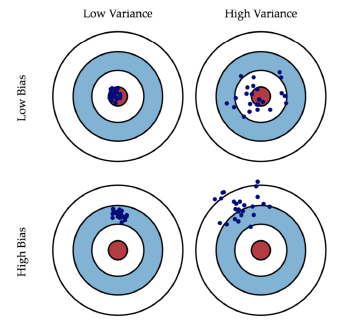
\includegraphics[width=\textwidth]{overfitting_cible}
\end{column}
\begin{column}{0.49\textwidth}
\begin{itemize}
\item The center of the target is a model that perfectly predicts the correct values!
\item We can repeat our entire model building process to get a number of separate hits on the target!

$\rightsquigarrow$ Each hit represents an \structure{individual realization of the model!}
\end{itemize}
\end{column}
\end{columns}
\begin{itemize}
\item Bias measures how far are in general these models' predictions are from the correct value!
\item  Variance is how much the predictions for a given point vary between different realizations of the model!
\end{itemize}
\end{frame}


\begin{frame}{Bias-Variance tradeoff}
\begin{itemize}
\item When do we have \alert{high bias}?
\begin{itemize}
\item  We have high bias when the model (function) cannot model the
true data distribution well!
\item   This doesn’t depend on the training data size!
\item   Underfitting!
\end{itemize}
\item When do we have \alert{high variance}?
\begin{itemize}
\item  We have high variance when there is a small amount of training
data and a very complex model!
\item   Overfitting!
\item  Variance decreases with larger training data, and increases with more complicated classifiers!
\end{itemize}
\end{itemize}
\end{frame}

\begin{frame}{Bias/Variance tradeoff}


\begin{figure}
\begin{center}
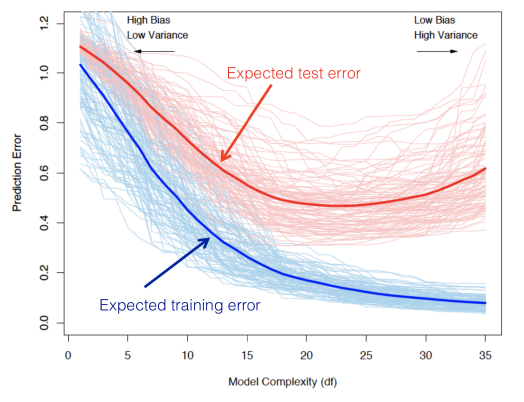
\includegraphics[width=0.8\textwidth]{overfitting_ex}
\end{center}
\end{figure}


\end{frame}

\begin{frame}{}

\begin{exampleblock}{\Large Take-home message}
{\Large
\begin{itemize}
\item   High bias $\Longrightarrow$ high training and test errors!
\item   High variance $\Longrightarrow$ low training error, high test errors!
\end{itemize}}
\end{exampleblock}

\end{frame}

% \begin{frame}{Model complexity}
% For instance, in regression, if the class of classifiers consists in trees, $\lambda$ is the tree depth, and it should not be chosen too high since noise could be also interpolated. 
% 
% \begin{block}{Model complexity}
% \begin{itemize}
%\item $\lambda$ small $\Rightarrow$ restrictive model $\Rightarrow$ bad fitting \\ 
%{\centering $\Rightarrow$ bias $\nearrow$, variance $\searrow$}
%\item $\lambda$ large $\Rightarrow$ flexible (complex) model $\Rightarrow$ overfitting \\ {\centering $\Rightarrow$ bias $\searrow$, variance $\nearrow$}
% \end{itemize}
% \end{block}
%
%\begin{alertblock}{Achtung!}
%A very good fitting on the training data (i.e. $f (X_i) = Y_i$ ) often implies poor predictive performances on new individuals. 
%\end{alertblock}
%
%\end{frame}

%\begin{frame}
%\begin{figure}
%\begin{center}
%\includegraphics[width=0.7\textwidth]{../../../ISUP2018/notes/img/overfitting.png}
%\caption{Overfitting can be detected by an increase in the test error.}
%\end{center}
%\end{figure}
%\end{frame}


\begin{frame}
\begin{figure}
\begin{center}
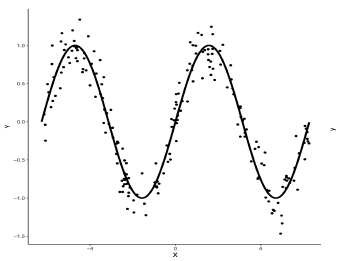
\includegraphics[width=0.49\textwidth]{overfitting_reg1.png}
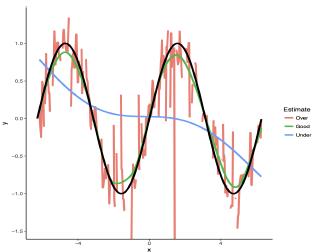
\includegraphics[width=0.49\textwidth]{overfitting_reg2.png}
\caption{Illustration of overfitting in regression. Here, $\lambda$ controls the regressor smoothness.}
\end{center}
\end{figure}
\end{frame}

%\begin{frame}
%\begin{figure}
%\begin{center}
%\includegraphics[width=0.7\textwidth]{../../../ISUP2018/notes/img/overfitting_classif.png}
%\caption{Illustration of overfitting in detection. Here, $\lambda$ controls the frontier smoothness.}
%\end{center}
%\end{figure}
%\end{frame}

 
\begin{frame}{A way to avoid overfitting}
\begin{block}{Penalization}
 Overfitting can also be prevented by penalization.
 \end{block}
  For instance, in linear regression, computing
  $$
  \hat{\beta}, \hat{e} \in \argmin_{\beta, e} \frac{1}{n} \sum_{i=1}^n \ell( Y_i, X_i^T \beta + e)
  $$
  could lead to bad classifier. Minimize instead 
    $$
  \hat{\beta}, \hat{e} \in \argmin_{\beta, e} \frac{1}{n} \sum_{i=1}^n \ell( Y_i, X_i^T \beta + e) + \lambda \mathrm{pen}(\beta)
  $$
  where $\mathrm{pen}$ is a penalization function, it forbids $\beta$ to be "too complex". $\lambda > 0$ is a tuning or smoothing parameter, that balances goodness-of-fit and penalization.
  \end{frame}




 \section{Cross-validation}
 
 \begin{frame}{Generalization}
 
\begin{block}{Goal of supervised learning}
\begin{itemize}
\item A trained classifier has to be generalizable: it must be able to work on other data than the training dataset
\item Generalizable means also “works without overfitting”. 
%\item This can be achieved using \structure{cross-validation}.
\end{itemize}
\end{block}
\begin{itemize}
\item The empirical error on the training set is a poor estimate of the generalization error (expected error on new data)!

$\rightsquigarrow$ If the model is overfitting, the generalization error can be arbitrarily large!
\item  We would like to estimate the generalization error on new data, which we do not have!
\end{itemize}

\begin{alertblock}{}
Any idea?
\end{alertblock}
\end{frame}
 

 \begin{frame}{Validation sets}
 \begin{itemize}
 \item Choose the model that performs best on a validation set separate from the training set!
 \begin{figure}
 \begin{center}
 %\includegraphics[width=0.8\textwidth]{img/hold_out}
 \end{center}
 \end{figure}
 \item Because we have not used the validation data at any point during training, the validation set can be considered “new data” and \structure{the error on the validation set is an estimation of the generalization error!}
 \end{itemize}
 \end{frame}
 \begin{frame}{Validation hold out}
 The simplest approach consists in splitting the data $\Dc_n$ into:
 \begin{enumerate}
 \item a learning or training set $\Dc_{n,train}$ used to learn the machine $f_n$,
\item a validation or test set $\Dc_{n,test}$ used to estimate the risk of $f_n$.
\end{enumerate}

\begin{algorithm}[H]
Inputs: $\Dc_n$ data, $(\Tc,\Vc)$ a partition of $\{1,\hdots , n\}$.
\begin{enumerate}
\item Learn the machine with $\Dc_{n,train} = \{ (X_i,Y_i), i \in \Tc\} \Longrightarrow f_{n,train}$;
\item Compute 
$$
\widehat{\Rc}_n (f_{n,train}) = \frac{1}{|\Vc|} \sum_{i\in \Vc} \ell \left( Y_i, f_{n,train}(X_i)\right).
$$
\end{enumerate}
\caption{Validation hold out}
\end{algorithm}

\begin{remark}
$n_{train} = |\Tc|$ and $n_{test}$ should be large enough.
\end{remark}
\end{frame}


%\begin{frame}{K-fold cross validation}
%
%\begin{itemize}
%\item Idea:  repeat the validation hold out described above on each element of a data partition
%\item Can be good specially when $n$ is small
%\item Let $\lambda \equiv$  the model complexity.
%\item  Assume that $\lambda$ lives in a \textbf{discrete set}. 
%\end{itemize}
%
%
%
%\begin{figure}[H]
%\begin{center}
%\includegraphics[width=4cm]{../../../ISUP2018/notes/img/k-foldCV.png}
%\end{center}
%\end{figure}
%
%\end{frame}


\begin{frame}{Model selection}
\begin{itemize}
\item What if we want to choose among k models?!
\begin{itemize}
\item  Train each model on the train set!
\item   Compute the prediction error of each model on the validation set!
\item Pick the model with the smallest prediction error on the validation set!
\end{itemize}
\item What is the generalization error?!
\begin{itemize}
\item  We don’t know!!
\item  Validation data was used to select the model!
\item   We have “cheated” and looked at the validation data: it is not a good proxy for new, unseen data any more!
\end{itemize}
\end{itemize}
\end{frame}

\begin{frame}{Model selection}
\begin{itemize}
\item Hence we need to set aside part of the data, the test set, that remains untouched during the entire procedure and on which we’ll estimate the generalization error!
\end{itemize}
\begin{exampleblock}{}
\begin{itemize}
\item Model selection: pick the best model!
\item Model assessment: estimate its prediction error on new data!
\end{itemize}
\end{exampleblock}
%\begin{figure}
%\begin{center}
%\includegraphics[width=9cm]{img/validation_set}
%\end{center}
%\end{figure}
\end{frame}

\begin{frame}{Validation sets}
\begin{itemize}
\item How much data should go in each of the training, validation and test sets?!
\item   How do we know that we have enough data to evaluate the prediction and generalization errors?!
\item  Empirical evaluation with sample re-use!
\begin{itemize}
\item  Cross-validation
\item  Bootstrap (random sampling with replacement)
\end{itemize}
\end{itemize}
\end{frame}

\begin{frame}{Cross-validation}
\begin{itemize}
\item Cut the training set in $K$ separate folds!
\item  For each fold, train on the $(K-1)$ remaining folds!
\end{itemize}
\begin{figure}
\begin{center}
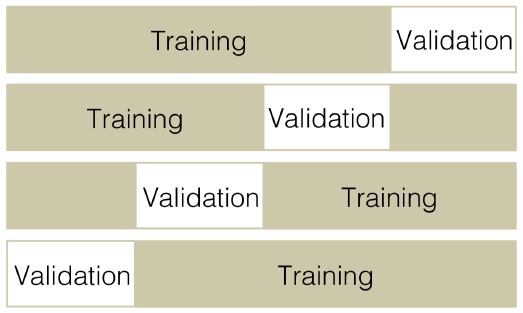
\includegraphics[width=8cm]{k-fold}
\end{center}
\end{figure}

\end{frame}

\begin{frame}{K-fold cross validation}


\begin{algorithm}[H]
Inputs: $\Dc_n$ data, $K$ an integer;
\begin{enumerate}
\item Define a random partition $\{\Ic_1,\hdots , \Ic_K\}$  of $\{1,\hdots , n\}$;
\item For a fixed $\lambda$, for $k=1,\hdots, K$
\begin{itemize}
\item $\Ic_{train} = \{1,\hdots , n \} \setminus \Ic_k \, \, $ and $\, \, \Ic_{test} = \Ic_k$ ; 
\item Learn the machine with $\Dc_{n,train} = \{ (X_i,Y_i), i \in \Tc\} \Longrightarrow f_{n,k}^{(\lambda)}$;
\item Compute the test error $\mathrm{Err}_{test} ( f_{n,k}^{(\lambda)} ) = \frac{1}{ n- | \Ic_k |} \sum_{i \in  \Ic_k} \ell \left( Y_i , f_{n,k}^{(\lambda)}( X_i ) \right)$.
\end{itemize}
\item Choose
$$\hat{\lambda}^{(CV)} \in \argmin_{\lambda \in \Lambda} \frac{1}{K} \sum_{k=1}^K \mathrm{Err}_{test} ( f_{n,k}^{(\lambda)} ).
$$
\end{enumerate} 
\caption{K-fold CV}
\end{algorithm}


\end{frame}
 
 
 
\begin{frame}{K-fold CV}

\begin{itemize}
\item $K$ has to be chosen by the user. Usually $K=5$ or $10$.
\item Advantage of this method over repeated random sub-sampling (bootstrap) is that all observations are used for both training and validation, and each observation is used for validation exactly once.
\end{itemize}
 
 \begin{block}{Leave-one-out CV}
 \begin{itemize}
\item When $K = n$, we obtain the leave-one-out (LOO) cross validation, since at each iteration exactly one instance is left out of the training sample.

\item In general, the leave-one-out error is very costly to compute, since it requires training $n$ times on samples of size $n-1$, but for some algorithms it admits a very efficient computation.

\item Exercise: LOO-CV in least squares regression
\end{itemize}
\end{block}

\end{frame}



\end{document}